\section{Important Concepts}
\label{concepts:sec}

\begin{definition}{\bf [Property Relation (PropRel)]}
Property relation represents the relationships between a variable and
its fields or methods to which the variable can access or call.
%when implementing a certa in task in a function.
\end{definition}

%\end{Pro_Rel}

A property relation between a variable \texttt{v} and its
property \texttt{p} is denoted by a triple $(v, p, t)$, 
where \texttt{t} is the type of relation, which can be 
either \texttt{fieldAccess} or \texttt{methodCall}.
In Figure~\ref{example_sim}, a set of property relations for \texttt{r}
includes $( \texttt{r}, \texttt{types}, \texttt{fieldAccess})$,
$( \texttt{r}, \texttt{getData}, \texttt{fieldAccess})$,
$( \texttt{r}, \texttt{getData()}, \texttt{methodCall})$.

\begin{definition}{\bf [Role Relation (RoleRel)]}
  Role relation represents the relationships between a variable and
  the method calls or field accesses in its usages.
\end{definition}

Since the names of methods or fields are not minified, we consider
them as the pivots in the usage context for recovering names of the
minified variables.
%
We focus on the roles of a variable used {\em as an argument in a method call}
 or {\em receiving the value returned by a method call or field access}.
%
If we have $o.m(...,v,...)$, $v = o.m(...)$, or $v = o.f$,
%where $m$ is a method call and $f$ is a field access,
then there exist
the role relations between $v$ and $m$, and between $v$ and $f$. The
rationale is that the names of $m$ and its argument are often in
conformance with each other, \eg
\texttt{getData(contentType)}. Similar rationale is applied to the
above assignments to $v$.

%A variable could be received a value of a field/method, or could be a
%input of an method invocation. For instance, in
%figure \ref{example_sim}, variable \texttt{r} receives the result of
%an assignment to the boolean expression $t.clipboardData ||
%a.clipboardData || e.dataTransfer$. In case of variable \texttt{f}, it
%is an argument of function \texttt{getData()} and the value
%of \texttt{getData()} is influenced by \texttt{f}.

A role relation between a variable \texttt{v} and a field/method
\texttt{p} is denoted by a triple $(v, p, t)$, where
\texttt{t} is the type of role relation. A role relation could
be either \texttt{argument} or \texttt{assignment}.

%We expect this role relation to contribute significantly to the name
%recovery process.
%%
%%This type of relation also contributes remarkably in reducing the name
%%searching space when recovering a variable.
%For example, a variable \texttt{x} in a minified code is assigned with
%the value of a field access to \texttt{httpBody} and is used as an
%argument in a call to \texttt{setBodyHttp()}. In our dataset, there
%are only 19 variable names that are assigned with the value
%of \texttt{httpBody}, while the number
%%of variable names is used for method call
%with regard to \texttt{setBodyHttp()} is 11.
%%The figure for names having both two relations is only 5.
%Then, there are only 5 candidate names that satisfy both conditions.
%Thus, our algorithm could reduce the number of candidates from +200K
%to only 5.
%%Therefore, the number of variable names could be recovered
%%for \texttt{x} reduced down to 5 in comparison with about 200k
%%variable names of our corpus.



%In our scope, we consider 2 common data dependency between
%variable \texttt{x} with fields, methods, which is shown in
%table \ref{table:DataDep} as below.

%\begin{table}[h!]
%\begin{tabular}{|c|c|c|c| }
% \hline Sample & Variable & Methods/Fields & Dependency Type \\
% [0.5ex] \hline x = Http.httpBody & x & httpBody &
% Assignment \\ \hline t.setBodyHttp(x) & x & setBodyHttp() &
% Argument \\ \hline
%\end{tabular}
%\caption{Data dependency}
%\label{table:DataDep}
%\end{table}


\begin{definition}{\bf [Relation Graph]}
A relation graph (RG) for a variable $v$ is a directed graph
in the shape of a star to represent the single-variable usage context
of $v$ with regard to its property and role relations with 
the fields and methods in its usage.
%
The center vertex of the RG represents the variable. The other vertices
represent the methods/fields in method calls or field accesses, respectively, and are labeled with their names. 
Edges represent relations and are labeled with relation types. 
\end{definition}

Figure~\ref{SG_sample_ano} shows the relation graph of the variable
\texttt{r}, which includes a set of property relations:
$( \texttt{r}, \texttt{types}, \texttt{fieldAccess})$, $( \texttt{r},
\texttt{getData}, \texttt{fieldAccess})$, $( \texttt{r},
\texttt{getData()}, \texttt{methodCall})$,
%
and a set of role relations: $( \texttt{r}, \texttt{clipboardData},
\texttt{assignment})$, $( \texttt{r}, \texttt{dataTransfer},
\texttt{assignment})$ in our example.

\begin{figure}[t]
	\begin{center}
		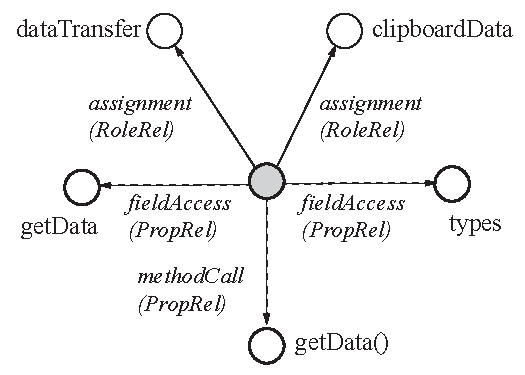
\includegraphics[width=.7\columnwidth]{figures/stargraph.pdf}
		\caption{The Relation Graph of Variable $r$ in Figure~\ref{example_sim}}
		\label{SG_sample_ano}
	\end{center}
\end{figure}
